% chap2.tex
\part{유지보수 및 신기술 적용}
\label{part:module}

% ---------------------------------------------------------------------------- %
%                                  NEW SECTION                                 %
% ---------------------------------------------------------------------------- %

\chapter{pyGRsim 모듈}

% ---------------------------------------------------------------------------- %
%                                  NEW SECTION                                 %
% ---------------------------------------------------------------------------- %

\section{pyGRsim 구조별 상세}
pyGRsim이랑 dragon이랑 launcher랑 나누어서 서술할 것임.

\subsection{pyGRsim}

\subsection{idragon}

% ---------------------------------------------------------------------------- %
%                                  NEW SECTION                                 %
% ---------------------------------------------------------------------------- %

\section{데이터 변환의 구현}
\subsection{grexcel to grjson}
...한 과정으로 이루어진다.

\subsection{grjson to GreenRetrofitModel}
...한 과정으로 이루어진다.

\subsection{GreenRetrofitModel to EnergyModel}
...한 과정으로 이루어진다.

\subsection{EnergyModel to idf}

\subsubsection{idf 기본 설정}
기본적으로 돌아가게 하기 위해서 아래 객체들을 먼저 만들어준다.

\subsubsection{DB류 객체들 내보내기}
material, construction, profile 들을 만들어준다.

\subsubsection{실재하는 객체들 하나씩 내보내기}
zone, surface, 설비같은 것들에 해당된다. 모든 EnergyModel 객체들은 다 to\_idf\_object 객체 가지고 있음. 기본적으로는 자기자신을 idfobject화 해서 계속 append하는 것이다.

\subsubsection{후처리}
...가 필요하다.

\subsubsection{ouptut 관리 등}
...가 필요하다.

% ---------------------------------------------------------------------------- %
%                                  NEW SECTION                                 %
% ---------------------------------------------------------------------------- %

\section{EnergyPlus의 실행}
외부에서 입력이 들어오면, 그림 \ref{fig:eplaunchbycode}\와 같이 EnergyPlus가 호출된다.
\begin{defaultfigure}
  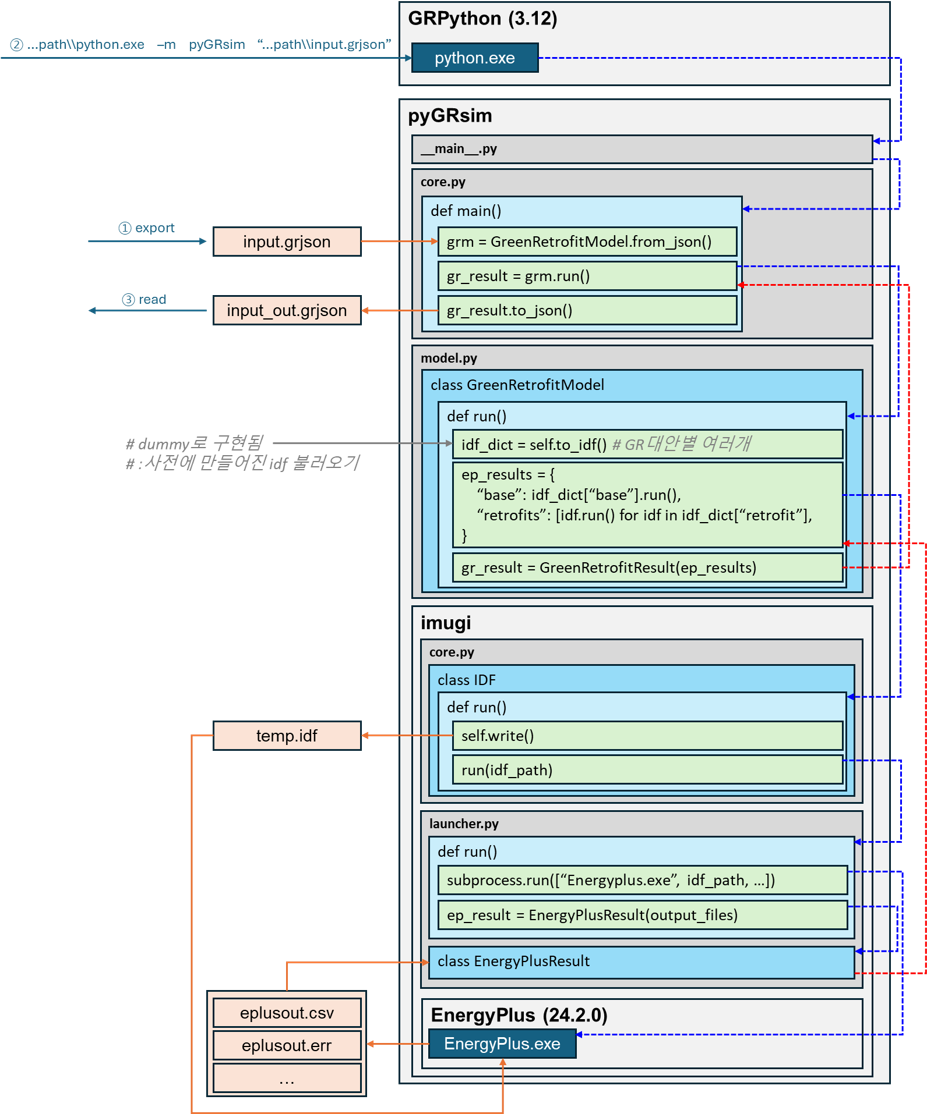
\includegraphics[height=0.99\textheight, width=\textwidth, keepaspectratio]{실행구조도.png}
  \caption{외부 호출 시 EnergyPlus launch되는 호출 흐름}
  \label{fig:eplaunchbycode}
\end{defaultfigure}

% ---------------------------------------------------------------------------- %
%                                  NEW SECTION                                 %
% ---------------------------------------------------------------------------- %

\section{예시코드}

% ---------------------------------------------------------------------------- %
%                                  NEW SECTION                                 %
% ---------------------------------------------------------------------------- %

\chapter{알고리즘의 수정과 코드의 유지보수}

\section{알고리즘의 수정 제안}

% ---------------------------------------------------------------------------- %
%                                  NEW SECTION                                 %
% ---------------------------------------------------------------------------- %

\section{기본값 변경}

% ---------------------------------------------------------------------------- %
%                                  NEW SECTION                                 %
% ---------------------------------------------------------------------------- %

\section{일반적인 코드의 유지보수}


% ---------------------------------------------------------------------------- %
%                                  NEW SECTION                                 %
% ---------------------------------------------------------------------------- %

\chapter{신기술 적용}

\section{신기술의 시뮬레이터 적용하기 위해 필요한 개념적인 과정}

% ---------------------------------------------------------------------------- %
%                                  NEW SECTION                                 %
% ---------------------------------------------------------------------------- %

\section{신기술을 본 시뮬레이터로 테스트해보는 방법}

idf에 모듈 형식으로 결합할 수 있도록 (즉, 독립적으로 추가될 수 있도록) 작성하여야 한다. 

% ---------------------------------------------------------------------------- %
%                                  NEW SECTION                                 %
% ---------------------------------------------------------------------------- %

\section{제도적으로 제출하기 위해 필요한 것}

이런 것들을 테스트하여 제출하면 평가가 가능하다.